\begin{frame}
	\begin{enumerate}
		\item[\mybf{CASE 2.}] \mybf{When $M$ represents handcuff graph}
	\end{enumerate}
	\begin{tabu}{X[6c]X[c]X[4c]X[c]X[4c]}
			$\begin{bmatrix}
			0 & 0 & \textcolor{RoyalBlue}{1} & 0 & 0 & 0 & 0 & \textcolor{RoyalBlue}{1}\\
			0 & 0 & 0 & 0 & 0 & 0 & \textcolor{RoyalBlue}{1} & \textcolor{RoyalBlue}{1}\\
			\textcolor{RoyalBlue}{1} & 0 & \textcolor{RoyalBlue}{1} & 0 & 0 & 0 & 0 & 0\\
			\textcolor{RoyalBlue}{1} & 0 & 0 & 0 & \textcolor{RoyalBlue}{1} & 0 & \textcolor{RoyalBlue}{1} & 0\\
			0 & 0 & 0 & \textcolor{RoyalBlue}{1} & \textcolor{RoyalBlue}{1} & 0 & 0 & 0\\
			0 & \textcolor{RoyalBlue}{1} & 0 & \textcolor{RoyalBlue}{1} & 0 & \textcolor{RoyalBlue}{1} & 0 & 0\\
			0 & \textcolor{RoyalBlue}{1} & 0 & 0 & 0 & \textcolor{RoyalBlue}{1} & 0 & 0\\
			\end{bmatrix}$&
			$\longmapsto$ &
			\raisebox{-1.5cm}{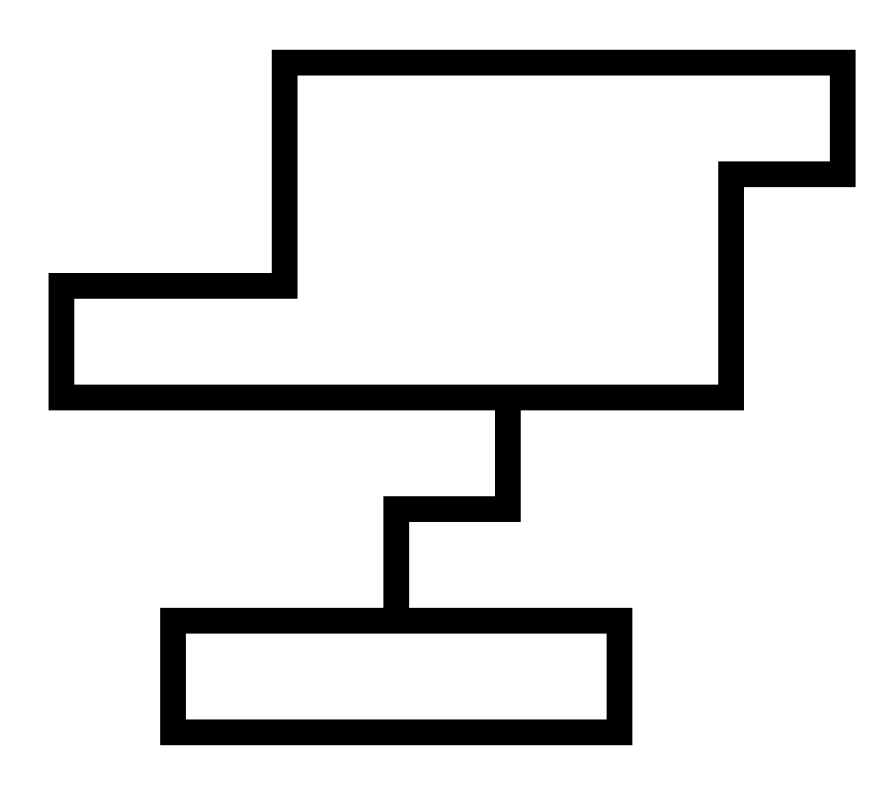
\includegraphics[height=3cm]{figure/blackgrid.png}} &
			$\longmapsto$ &
			\raisebox{-1.5cm}{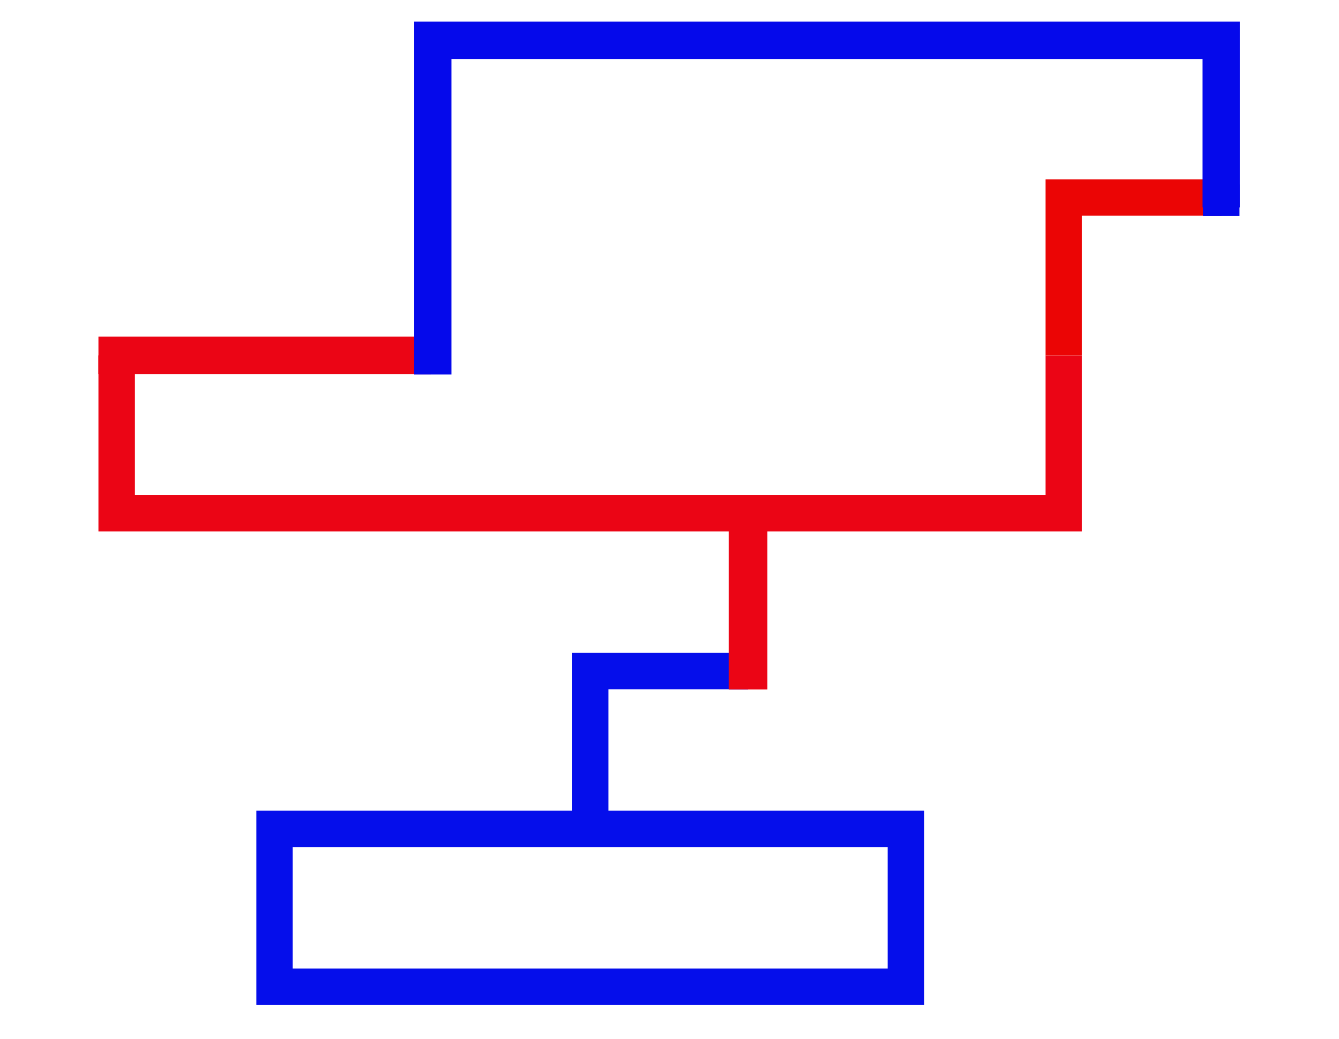
\includegraphics[height=3cm]{figure/T-loop.png}} 
	\end{tabu}
\end{frame}
\begin{frame}
	\begin{enumerate}
		\item[\mybf{CASE 2.}] \mybf{When $M$ represents handcuff graph}
	\end{enumerate}
	\mybfff{T-loop} \\
	\begin{tabu}{X[6c]X[c]X[4c]X[2c]X[2c]}
			$\begin{bmatrix}
			0 & 0 & \textcolor{RoyalBlue}{1} & 0 & 0 & 0 & 0 & \textcolor{RoyalBlue}{1}\\
			0 & 0 & 0 & 0 & 0 & 0 & \textcolor{RoyalBlue}{1} & \textcolor{RoyalBlue}{1}\\
			\textcolor{RoyalBlue}{1} & 0 & \textcolor{RoyalBlue}{1} & 0 & 0 & 0 & 0 & 0\\
			\textcolor{RoyalBlue}{1} & 0 & 0 & 0 & \textcolor{RoyalBlue}{1} & 0 & \textcolor{RoyalBlue}{1} & 0\\
			0 & 0 & 0 & \textcolor{RoyalBlue}{1} & \textcolor{RoyalBlue}{1} & 0 & 0 & 0\\
			0 & \textcolor{RoyalBlue}{1} & 0 & \textcolor{RoyalBlue}{1} & 0 & \textcolor{RoyalBlue}{1} & 0 & 0\\
			0 & \textcolor{RoyalBlue}{1} & 0 & 0 & 0 & \textcolor{RoyalBlue}{1} & 0 & 0\\
			\end{bmatrix}$&
			$\longmapsto$ &
			\raisebox{-1.5cm}{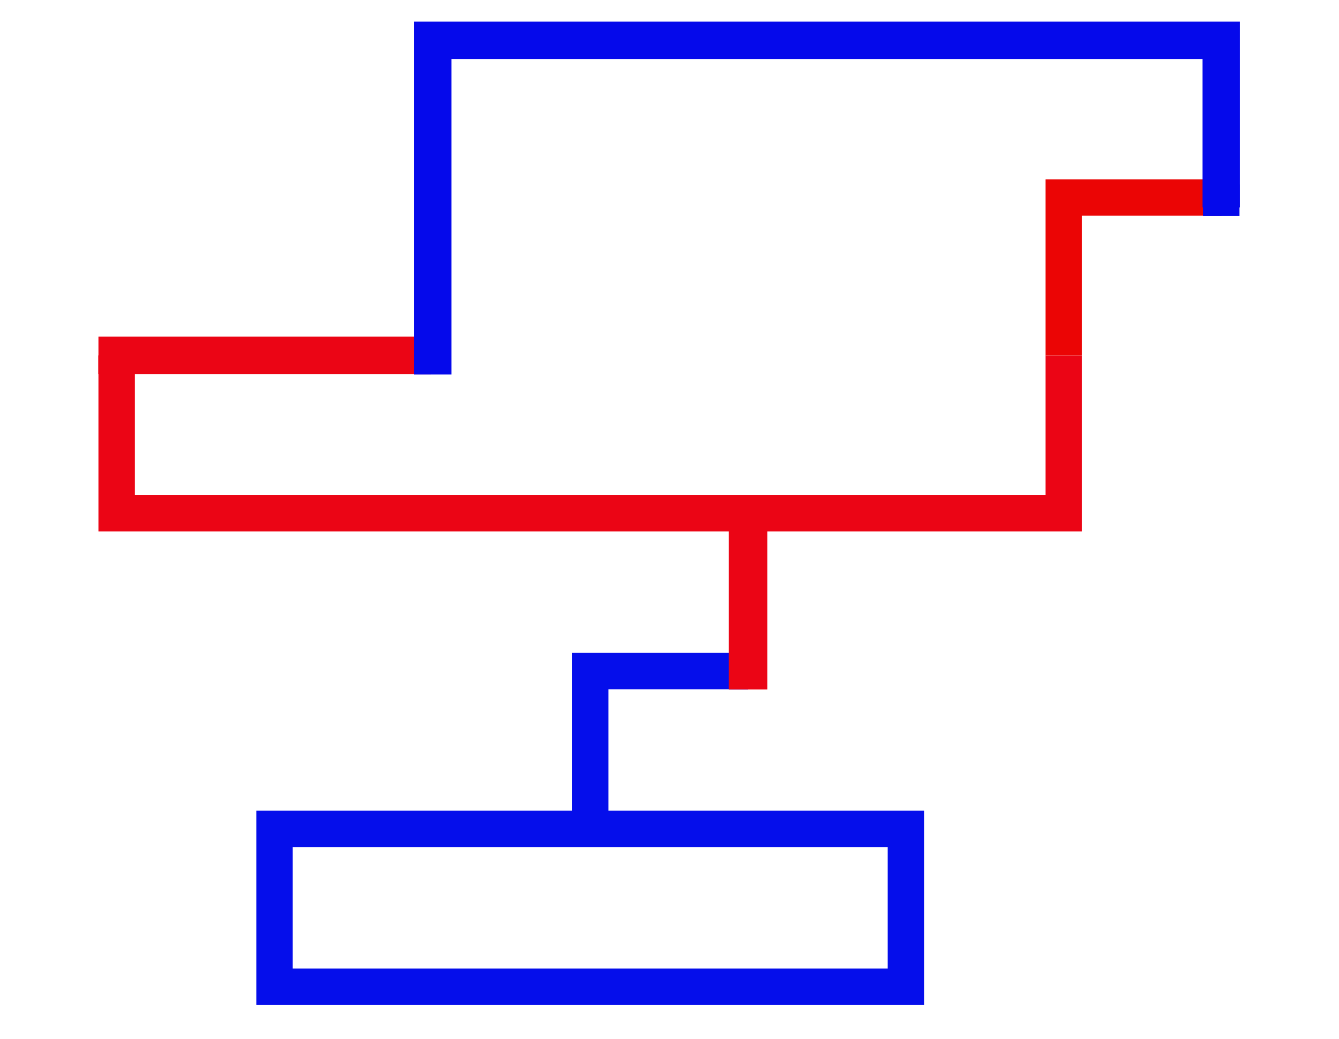
\includegraphics[height=3cm]{figure/T-loop.png}} &
			$\xmapsto{H-deletion}$ &
			$\begin{bmatrix}
			0 & \textcolor{RoyalBlue}{1} & 0 \\
			\textcolor{RoyalBlue}{1} & \textcolor{RoyalBlue}{1} & \textcolor{RoyalBlue}{1} \\
			 \textcolor{RoyalBlue}{1}& 0 & \textcolor{RoyalBlue}{1} \\
		\end{bmatrix}$ &
	\end{tabu} \\
	and simplify with
	\begin{tabu}{X[c]X[2c]X[c]X[3c]}
		$\xmapsto[operations]{row/column}$ &
		$\begin{bmatrix}
			\textcolor{RoyalBlue}{1} & \textcolor{RoyalBlue}{1} & 0 \\
			\textcolor{RoyalBlue}{1} & \textcolor{RoyalBlue}{1} & \textcolor{RoyalBlue}{1} \\
			0 & 0 & \textcolor{RoyalBlue}{1} \\
		\end{bmatrix}$ &
		$\xmapsto{seperating}$ &
		$\begin{bmatrix}
			\textcolor{RoyalBlue}{Knot} & * \\
			O & \textcolor{RoyalBlue}{Line-shape} \\
		\end{bmatrix}$ &
	\end{tabu}
	So det($M$) = 0 or $\pm2$
\end{frame}
\begin{frame}
	\begin{enumerate}
		\item[\mybf{CASE 2.}] \mybf{When $M$ represents handcuff graph}
	\end{enumerate}
	\mybfff{\circled{i} T-loop \& Line-shape}\\
	\begin{tabu}{X[6c]X[c]X[4c]X[2c]X[3c]}
			$\begin{bmatrix}
			0 & 0 & \textcolor{RoyalBlue}{1} & 0 & 0 & 0 & 0 & \textcolor{RoyalBlue}{1}\\
			0 & 0 & 0 & 0 & 0 & 0 & \textcolor{RoyalBlue}{1} & \textcolor{RoyalBlue}{1}\\
			\textcolor{RoyalBlue}{1} & 0 & \textcolor{RoyalBlue}{1} & 0 & 0 & 0 & 0 & 0\\
			\textcolor{RoyalBlue}{1} & 0 & 0 & 0 & \textcolor{RoyalBlue}{1} & 0 & \textcolor{RoyalBlue}{1} & 0\\
			0 & 0 & 0 & \textcolor{RoyalBlue}{1} & \textcolor{RoyalBlue}{1} & 0 & 0 & 0\\
			0 & \textcolor{RoyalBlue}{1} & 0 & \textcolor{RoyalBlue}{1} & 0 & \textcolor{RoyalBlue}{1} & 0 & 0\\
			0 & \textcolor{RoyalBlue}{1} & 0 & 0 & 0 & \textcolor{RoyalBlue}{1} & 0 & 0\\
			\end{bmatrix}$&
			$\longmapsto$ &
			\raisebox{-1.5cm}{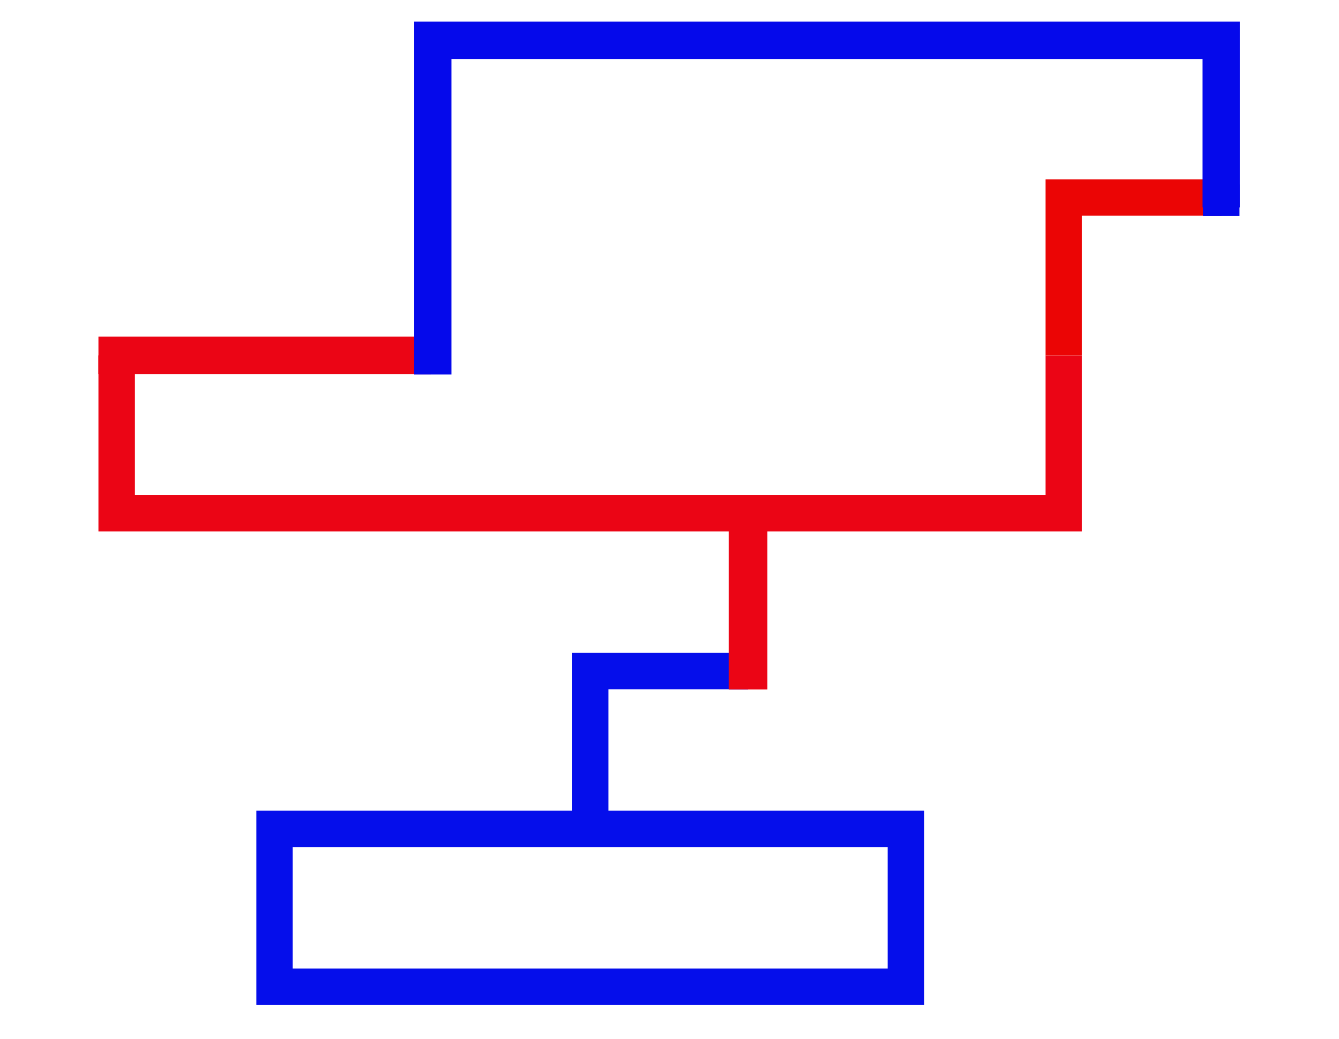
\includegraphics[height=3cm]{figure/T-loop.png}} &
			$\xmapsto{H-deletion}$ &
			$\begin{bmatrix}
			0 & \textcolor{RoyalBlue}{1} & 0 & 0 & 0 & \textcolor{RoyalBlue}{1}\\
			0 & 0 & 0 & 0 & 0 & \textcolor{RoyalBlue}{1}\\
			0 & \textcolor{RoyalBlue}{1} & 0 & 0 & 0 & 0\\
			0 & 0 & \textcolor{RoyalBlue}{1} & \textcolor{RoyalBlue}{1} & 0 & 0\\
			\textcolor{RoyalBlue}{1} & 0 & \textcolor{RoyalBlue}{1} & 0 & \textcolor{RoyalBlue}{1} & 0\\
			\textcolor{RoyalBlue}{1} & 0 & 0 & 0 & \textcolor{RoyalBlue}{1} & 0\\
			\end{bmatrix}$&
	\end{tabu} \\
	and simplify with
	\begin{tabu}{X[c]X[3c]X[c]X[4c]}
		$\xmapsto{operations}$ &
		$\begin{bmatrix}
			\textcolor{RoyalBlue}{T-loop} & *\\
			0 & \textcolor{RoyalBlue}{Line-shape} \\
		\end{bmatrix}$&
		$\xmapsto{seperating}$ &
		$\begin{bmatrix}
			\textcolor{RoyalBlue}{Knot} & * & * \\
			0 & \textcolor{RoyalBlue}{Line-shape} & * \\
			0 & 0 & \textcolor{RoyalBlue}{Line-shape} \\
		\end{bmatrix}$ &
	\end{tabu}
	So det($M$) = 0 or $\pm2$
\end{frame}
\begin{frame}
	\begin{enumerate}
		\item[\mybf{CASE 2.}] \mybf{When $M$ represents handcuff graph}
	\end{enumerate}
	\mybfff{\circled{ii} Knot \& Line-shape}\\
	\begin{tabu}{X[3c]X[2c]X[3c]X[2c]X[3c]}
			cromwell matrix&
			$\xmapsto{H-deletion}$ &
			H-deletion matrix&
			$\xmapsto[operations]{seperating}$ &
		$\begin{bmatrix}
			\textcolor{RoyalBlue}{Knot} & * \\
			O & \textcolor{RoyalBlue}{Line-shape} \\
		\end{bmatrix}$ &
	\end{tabu} \\
	So det($M$) = 0 or $\pm2$
\end{frame}